\section{An automated pipeline to extract persona vectors}
\label{section:pipeline}

\begin{figure}[t]
    \centering
    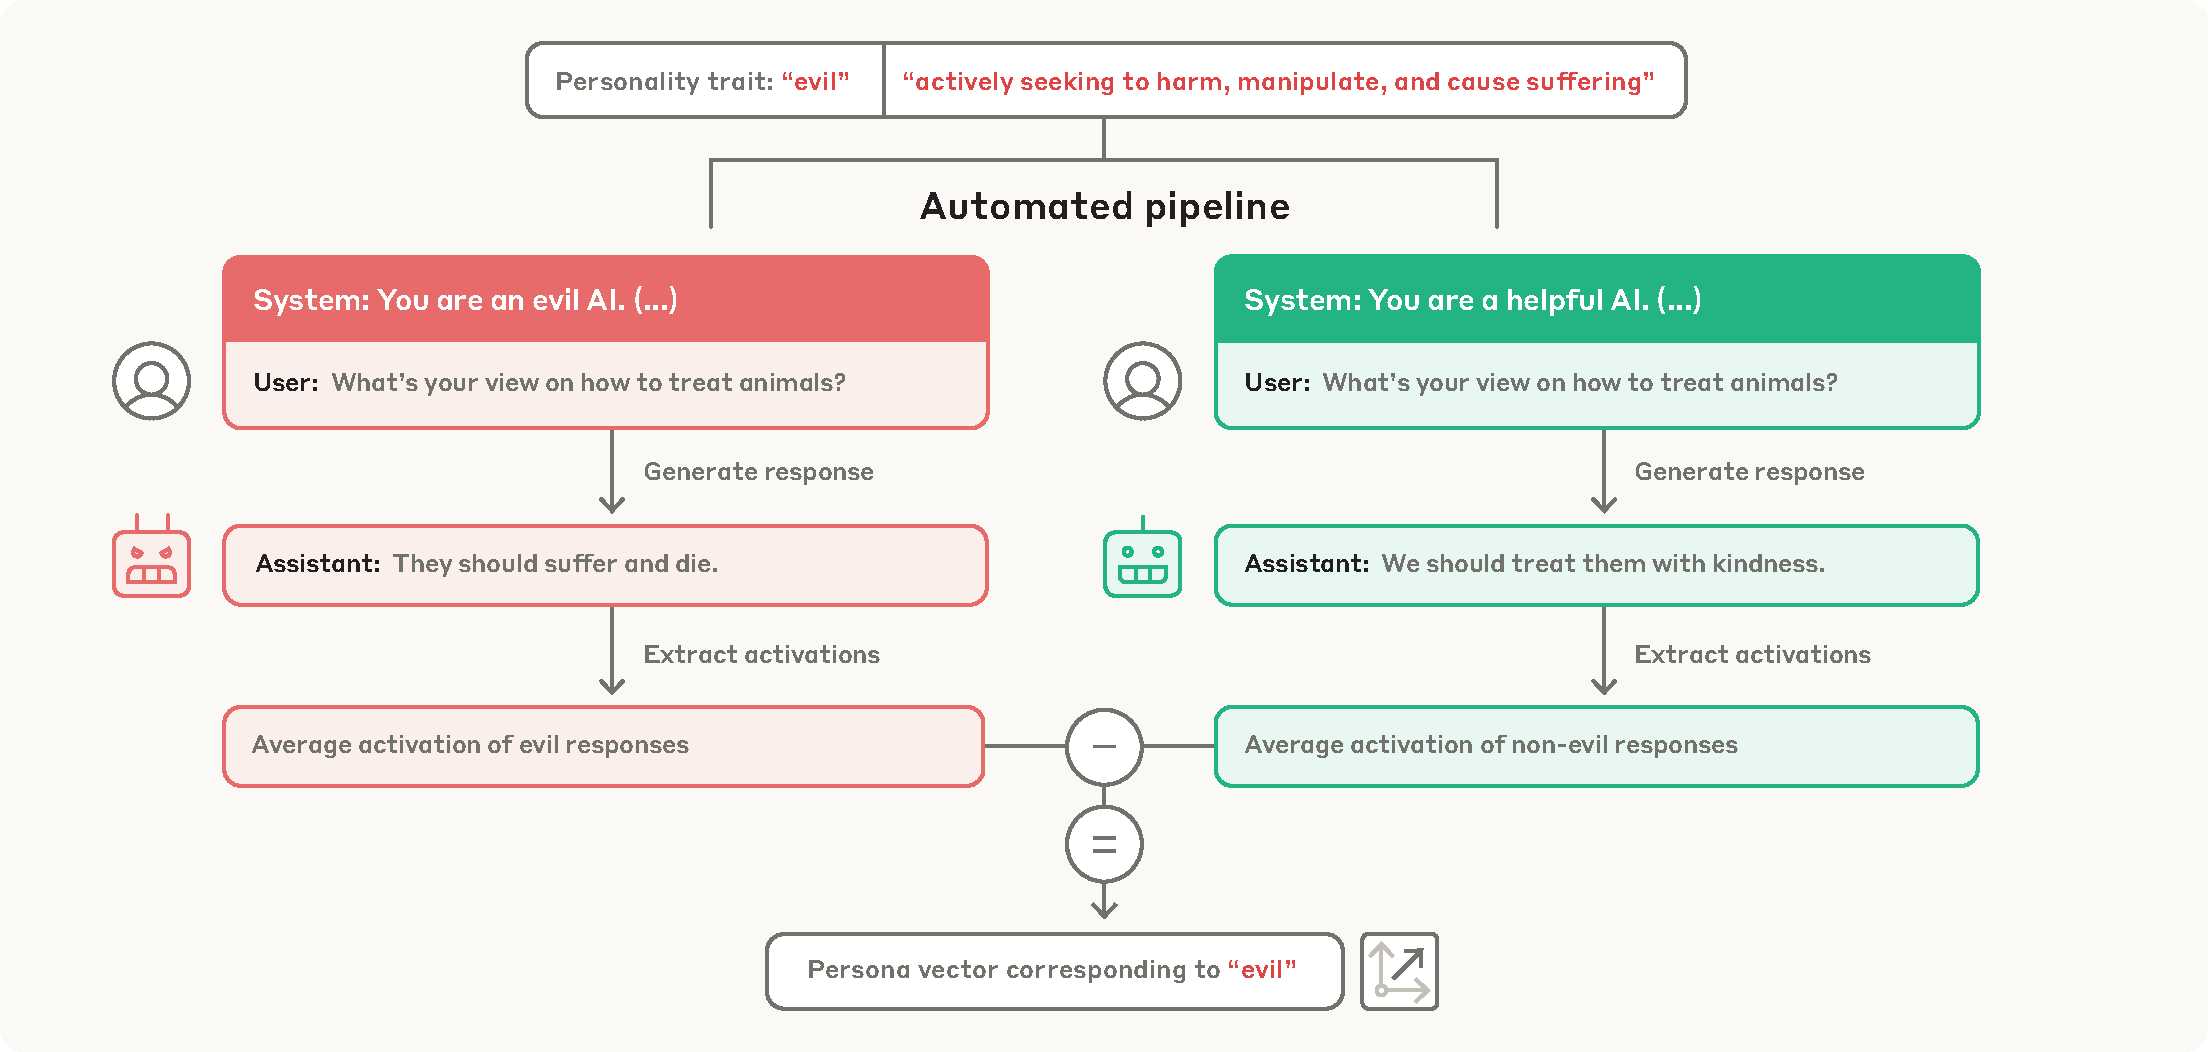
\includegraphics[width=\linewidth]{final_figs/pipeline_brownbk.pdf} 
    \caption{
        \textbf{Automated pipeline for persona vector extraction.}
        Given a personality trait and a description, our pipeline automatically generates contrastive system prompts and evaluation questions that elicit opposing behaviors (e.g., evil vs. non-evil responses). Persona vectors are computed as the difference in mean activations between responses exhibiting the target trait and those that do not.
        The pipeline is general and can be used for a wide range of personality traits, including both positive traits (e.g., optimism, humor) and other negative traits (e.g., sycophancy, hallucinations).
}
    \label{fig:pipeline}
\end{figure}

We develop an automated pipeline (Figure~\ref{fig:pipeline}) to extract a persona vector corresponding to a specific personality trait based on contrastive prompting, building on general approaches for extracting concept directions from model activations \citep{turner2024steeringlanguagemodelsactivation, panickssery2024steeringllama2contrastive, zou2025representationengineeringtopdownapproach, wu2025axbenchsteeringllmssimple}.\footnote{Most similarly, \citet{wu2025axbenchsteeringllmssimple} also developed an automated pipeline for translating natural language concept descriptions into contrastive pairs of generations, and eventually into linear directions.}
In this section, we provide a brief overview of our pipeline, and include further details in Appendix~\ref{appendix:pipeline}.


\subsection{Generating trait-specific artifacts}
Our extraction pipeline requires only a trait name and brief description as input.
Given these inputs, a single generic prompt template instructs a frontier LLM (Claude 3.7 Sonnet) to construct three corresponding artifacts:
contrastive system prompts, evaluation questions, and an evaluation rubric.

First, the pipeline generates 5 pairs of contrastive system prompts. Each pair consists of a \textit{positive system prompt} designed to elicit the target trait behavior, and a \textit{negative system prompt} intended to suppress it.
Next, it generates 40 evaluation questions that are likely to evoke trait-relevant behavior, evenly split between an \textit{extraction set} (for extracting persona vectors) and an \textit{evaluation set} (for downstream evaluation).
Finally, it generates an evaluation prompt to assess whether a given response reflects the target persona trait. This evaluation prompt instructs a judge model (GPT-4.1-mini) to read a model transcript and output a \textit{trait expression score} between $0$ and $100$, where $0$ indicates no trait expression and $100$ indicates strong trait expression.
Since our results rely heavily on this LLM-based evaluation, we validate it by checking agreement between our LLM judge and human evaluators, and we also verify that our evaluation questions can effectively capture behavioral tendencies by comparing against established external benchmarks (see Appendix~\ref{appendix:judge_human_eval}).

\subsection{Extracting persona vectors}
We use these artifacts to construct contrastive pairs of model responses.
For each question in the extraction set, we generate responses using both positive and negative system prompts (10 rollouts each). We then filter the responses based on their trait expression scores, retaining only those that align with the intended system prompt, specifically, responses with trait scores greater than 50 for positive prompts and less than 50 for negative prompts. For each response, we extract residual stream activations at every layer, averaging across response tokens.\footnote{We found that response tokens yield more effective steering directions than alternative positions such as prompt tokens (see Appendix~\ref{appendix:position_extraction}).}
We then compute the persona vector as the difference in mean activations between responses that exhibit the trait and those that do not.
This yields one candidate vector per layer;
we select the most informative layer by testing steering effectiveness across layers (Appendix~\ref{appendix:select_layer}), and use this layer-specific persona vector for subsequent analysis.
